\documentclass{ximera}  


%\usepackage{todonotes}
%\usepackage{mathtools} %% Required for wide table Curl and Greens
%\usepackage{cuted} %% Required for wide table Curl and Greens
\newcommand{\todo}{}

\usepackage{esint} % for \oiint
\ifxake%%https://math.meta.stackexchange.com/questions/9973/how-do-you-render-a-closed-surface-double-integral
\renewcommand{\oiint}{{\large\bigcirc}\kern-1.56em\iint}
\fi


\graphicspath{
  {./}
  {jpg}
  {ximeraTutorial/}
  {basicPhilosophy/}
  {functionsOfSeveralVariables/}
  {normalVectors/}
  {lagrangeMultipliers/}
  {vectorFields/}
  {greensTheorem/}
  {shapeOfThingsToCome/}
  {dotProducts/}
  {partialDerivativesAndTheGradientVector/}
  {../productAndQuotientRules/exercises/}
  {../motionAndPathsInSpace/exercises/}
  {../normalVectors/exercisesParametricPlots/}
  {../continuityOfFunctionsOfSeveralVariables/exercises/}
  {../partialDerivativesAndTheGradientVector/exercises/}
  {../directionalDerivativeAndChainRule/exercises/}
  {../commonCoordinates/exercisesCylindricalCoordinates/}
  {../commonCoordinates/exercisesSphericalCoordinates/}
  {../greensTheorem/exercisesCurlAndLineIntegrals/}
  {../greensTheorem/exercisesDivergenceAndLineIntegrals/}
  {../shapeOfThingsToCome/exercisesDivergenceTheorem/}
  {../greensTheorem/}
  {../shapeOfThingsToCome/}
  {../separableDifferentialEquations/exercises/}
  {vectorFields/}
}

\newcommand{\mooculus}{\textsf{\textbf{MOOC}\textnormal{\textsf{ULUS}}}}

\usepackage{tkz-euclide}\usepackage{tikz}
\usepackage{tikz-cd}
\usetikzlibrary{arrows}
\tikzset{>=stealth,commutative diagrams/.cd,
  arrow style=tikz,diagrams={>=stealth}} %% cool arrow head
\tikzset{shorten <>/.style={ shorten >=#1, shorten <=#1 } } %% allows shorter vectors

\usetikzlibrary{backgrounds} %% for boxes around graphs
\usetikzlibrary{shapes,positioning}  %% Clouds and stars
\usetikzlibrary{matrix} %% for matrix
\usepgfplotslibrary{polar} %% for polar plots
\usepgfplotslibrary{fillbetween} %% to shade area between curves in TikZ
\usetkzobj{all}
\usepackage[makeroom]{cancel} %% for strike outs
%\usepackage{mathtools} %% for pretty underbrace % Breaks Ximera
%\usepackage{multicol}
\usepackage{pgffor} %% required for integral for loops



%% http://tex.stackexchange.com/questions/66490/drawing-a-tikz-arc-specifying-the-center
%% Draws beach ball
\tikzset{pics/carc/.style args={#1:#2:#3}{code={\draw[pic actions] (#1:#3) arc(#1:#2:#3);}}}



\usepackage{array}
\setlength{\extrarowheight}{+.1cm}
\newdimen\digitwidth
\settowidth\digitwidth{9}
\def\divrule#1#2{
\noalign{\moveright#1\digitwidth
\vbox{\hrule width#2\digitwidth}}}





\newcommand{\RR}{\mathbb R}
\newcommand{\R}{\mathbb R}
\newcommand{\N}{\mathbb N}
\newcommand{\Z}{\mathbb Z}

\newcommand{\sagemath}{\textsf{SageMath}}


%\renewcommand{\d}{\,d\!}
\renewcommand{\d}{\mathop{}\!d}
\newcommand{\dd}[2][]{\frac{\d #1}{\d #2}}
\newcommand{\pp}[2][]{\frac{\partial #1}{\partial #2}}
\renewcommand{\l}{\ell}
\newcommand{\ddx}{\frac{d}{\d x}}

\newcommand{\zeroOverZero}{\ensuremath{\boldsymbol{\tfrac{0}{0}}}}
\newcommand{\inftyOverInfty}{\ensuremath{\boldsymbol{\tfrac{\infty}{\infty}}}}
\newcommand{\zeroOverInfty}{\ensuremath{\boldsymbol{\tfrac{0}{\infty}}}}
\newcommand{\zeroTimesInfty}{\ensuremath{\small\boldsymbol{0\cdot \infty}}}
\newcommand{\inftyMinusInfty}{\ensuremath{\small\boldsymbol{\infty - \infty}}}
\newcommand{\oneToInfty}{\ensuremath{\boldsymbol{1^\infty}}}
\newcommand{\zeroToZero}{\ensuremath{\boldsymbol{0^0}}}
\newcommand{\inftyToZero}{\ensuremath{\boldsymbol{\infty^0}}}



\newcommand{\numOverZero}{\ensuremath{\boldsymbol{\tfrac{\#}{0}}}}
\newcommand{\dfn}{\textbf}
%\newcommand{\unit}{\,\mathrm}
\newcommand{\unit}{\mathop{}\!\mathrm}
\newcommand{\eval}[1]{\bigg[ #1 \bigg]}
\newcommand{\seq}[1]{\left( #1 \right)}
\renewcommand{\epsilon}{\varepsilon}
\renewcommand{\phi}{\varphi}


\renewcommand{\iff}{\Leftrightarrow}

\DeclareMathOperator{\arccot}{arccot}
\DeclareMathOperator{\arcsec}{arcsec}
\DeclareMathOperator{\arccsc}{arccsc}
\DeclareMathOperator{\si}{Si}
\DeclareMathOperator{\scal}{scal}
\DeclareMathOperator{\sign}{sign}


%% \newcommand{\tightoverset}[2]{% for arrow vec
%%   \mathop{#2}\limits^{\vbox to -.5ex{\kern-0.75ex\hbox{$#1$}\vss}}}
\newcommand{\arrowvec}[1]{{\overset{\rightharpoonup}{#1}}}
%\renewcommand{\vec}[1]{\arrowvec{\mathbf{#1}}}
\renewcommand{\vec}[1]{{\overset{\boldsymbol{\rightharpoonup}}{\mathbf{#1}}}\hspace{0in}}

\newcommand{\point}[1]{\left(#1\right)} %this allows \vector{ to be changed to \vector{ with a quick find and replace
\newcommand{\pt}[1]{\mathbf{#1}} %this allows \vec{ to be changed to \vec{ with a quick find and replace
\newcommand{\Lim}[2]{\lim_{\point{#1} \to \point{#2}}} %Bart, I changed this to point since I want to use it.  It runs through both of the exercise and exerciseE files in limits section, which is why it was in each document to start with.

\DeclareMathOperator{\proj}{\mathbf{proj}}
\newcommand{\veci}{{\boldsymbol{\hat{\imath}}}}
\newcommand{\vecj}{{\boldsymbol{\hat{\jmath}}}}
\newcommand{\veck}{{\boldsymbol{\hat{k}}}}
\newcommand{\vecl}{\vec{\boldsymbol{\l}}}
\newcommand{\uvec}[1]{\mathbf{\hat{#1}}}
\newcommand{\utan}{\mathbf{\hat{t}}}
\newcommand{\unormal}{\mathbf{\hat{n}}}
\newcommand{\ubinormal}{\mathbf{\hat{b}}}

\newcommand{\dotp}{\bullet}
\newcommand{\cross}{\boldsymbol\times}
\newcommand{\grad}{\boldsymbol\nabla}
\newcommand{\divergence}{\grad\dotp}
\newcommand{\curl}{\grad\cross}
%\DeclareMathOperator{\divergence}{divergence}
%\DeclareMathOperator{\curl}[1]{\grad\cross #1}
\newcommand{\lto}{\mathop{\longrightarrow\,}\limits}

\renewcommand{\bar}{\overline}

\colorlet{textColor}{black}
\colorlet{background}{white}
\colorlet{penColor}{blue!50!black} % Color of a curve in a plot
\colorlet{penColor2}{red!50!black}% Color of a curve in a plot
\colorlet{penColor3}{red!50!blue} % Color of a curve in a plot
\colorlet{penColor4}{green!50!black} % Color of a curve in a plot
\colorlet{penColor5}{orange!80!black} % Color of a curve in a plot
\colorlet{penColor6}{yellow!70!black} % Color of a curve in a plot
\colorlet{fill1}{penColor!20} % Color of fill in a plot
\colorlet{fill2}{penColor2!20} % Color of fill in a plot
\colorlet{fillp}{fill1} % Color of positive area
\colorlet{filln}{penColor2!20} % Color of negative area
\colorlet{fill3}{penColor3!20} % Fill
\colorlet{fill4}{penColor4!20} % Fill
\colorlet{fill5}{penColor5!20} % Fill
\colorlet{gridColor}{gray!50} % Color of grid in a plot

\newcommand{\surfaceColor}{violet}
\newcommand{\surfaceColorTwo}{redyellow}
\newcommand{\sliceColor}{greenyellow}




\pgfmathdeclarefunction{gauss}{2}{% gives gaussian
  \pgfmathparse{1/(#2*sqrt(2*pi))*exp(-((x-#1)^2)/(2*#2^2))}%
}


%%%%%%%%%%%%%
%% Vectors
%%%%%%%%%%%%%

%% Simple horiz vectors
\renewcommand{\vector}[1]{\left\langle #1\right\rangle}


%% %% Complex Horiz Vectors with angle brackets
%% \makeatletter
%% \renewcommand{\vector}[2][ , ]{\left\langle%
%%   \def\nextitem{\def\nextitem{#1}}%
%%   \@for \el:=#2\do{\nextitem\el}\right\rangle%
%% }
%% \makeatother

%% %% Vertical Vectors
%% \def\vector#1{\begin{bmatrix}\vecListA#1,,\end{bmatrix}}
%% \def\vecListA#1,{\if,#1,\else #1\cr \expandafter \vecListA \fi}

%%%%%%%%%%%%%
%% End of vectors
%%%%%%%%%%%%%

%\newcommand{\fullwidth}{}
%\newcommand{\normalwidth}{}



%% makes a snazzy t-chart for evaluating functions
%\newenvironment{tchart}{\rowcolors{2}{}{background!90!textColor}\array}{\endarray}

%%This is to help with formatting on future title pages.
\newenvironment{sectionOutcomes}{}{}



%% Flowchart stuff
%\tikzstyle{startstop} = [rectangle, rounded corners, minimum width=3cm, minimum height=1cm,text centered, draw=black]
%\tikzstyle{question} = [rectangle, minimum width=3cm, minimum height=1cm, text centered, draw=black]
%\tikzstyle{decision} = [trapezium, trapezium left angle=70, trapezium right angle=110, minimum width=3cm, minimum height=1cm, text centered, draw=black]
%\tikzstyle{question} = [rectangle, rounded corners, minimum width=3cm, minimum height=1cm,text centered, draw=black]
%\tikzstyle{process} = [rectangle, minimum width=3cm, minimum height=1cm, text centered, draw=black]
%\tikzstyle{decision} = [trapezium, trapezium left angle=70, trapezium right angle=110, minimum width=3cm, minimum height=1cm, text centered, draw=black]




 
\title{Capacitance} 
\author{Milica Markovic} 
\outcome{Define capacitance. Derive capacitance of simple symetrical structures.}
\begin{document}  
\begin{abstract}  

\end{abstract}  
\maketitle    


\section{What is Capacitance?}
Capacitance is a constant that relates the amount of charge on a conductor with a potential difference between conductors. Whenever we have two conductors at different potentials, separated by an insulator (dielectric), there will be electric field between them, and we can define the ability for those two conductors to store charge. This is called a capacitance.

\begin{equation}
C=\frac{Q}{V}
\end{equation}

From Gauss's law, we found that the electric field is proportional to the charge enclosed $Q \sim E$. The capacitance therefore represents the strenght of the electric field around a conductor for a fixed voltage between the conductors. If we for example have two sets of conductors, for the same voltage between them the electric field will be stronger around the conductor set with higher capacitance, and this conductor set will have higher ability to store charge. It will store more charge for the same voltage difference than the other conductor set.

Capacitance relates the current with the change in voltage. The current is defined as the change of charge in time  $i=\frac{dq}{dt}$. Since charge is from the above equation equal to the product of capacitance and voltage, Q=CV, then the current is proportional to the change in voltage. If the voltage changes twice as fast, the current doubles. The voltage V is the potential  difference between the positive and negative plate of the capacitor. 

\begin{equation}
i=C \frac{dv}{dt}
\end{equation}


\section{Computing Capacitance}

Capacitance can be computed:

\begin{enumerate}
\item from its definition $C=\frac{Q}{V}$. You can first apply Gauss's law to find the electric field, then find the potential difference between the conductors. The potential difference depends on charge, and so, the charges will cancel.
\item from the expression for the electrostatic energy $W_e=\frac{1}{2} \int_V  \epsilon_o \epsilon_r E^2 \, \,dV$. First apply Gauss's law to find the electric field E, square it, and integrate throughout the volume enclosed by the two conductors. 
\end{enumerate}


\section{Capacitors}

Capacitors are components that provide capacitance in electronic circuits. They are used in filters, PCB power-distribution networks, matching circuits, delay lines etc. Typical capacitors are shown in Figure \ref{fig:capacitors}. Earth is a conductor, so any conductor either on it's own or in pair with another conductor can be modeled as a capacitor. For a single conductor, for example a metallic conductor in air, the other "conductor" is earth, or another nearby metallic object. Transmission lines have two conductors, a "signal" and "ground" conductor, so they have capacitance per unit lenght, and we can model them with a distributed capacitors. In this section, using Maxwell's equations, we will derive equations for capacitance for typical capacitors and transmission lines.


\begin{figure}[htbp]
\begin{center}
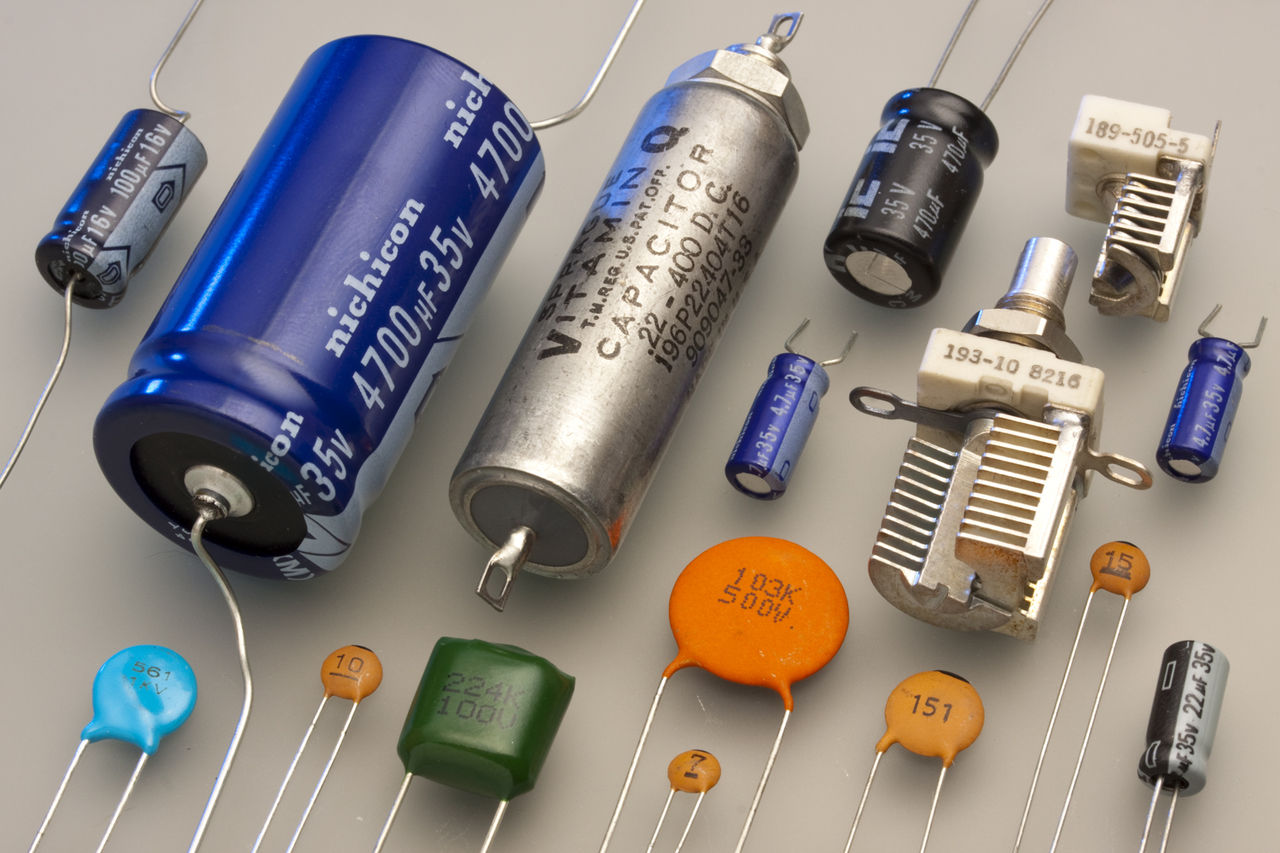
\includegraphics[scale=0.8]{../jpg/capacitors.jpg}
\end{center}
\caption{\href{https://en.wikipedia.org/wiki/Capacitor}{Various commercially available capacitors. Reference: Wikipedia}}\label{fig:capacitors}
\end{figure}


\section{Analysis of a Parallel-Plate Capacitor with a homogeneous dielectric}


A parallel plate capacitor consists of two conductive plates, as shown in Figure \ref{fig:ParallePlateCapacitorPlain}. The surface area of the plates is S and the charge on each plate is Q. The plates are separated by a distance d ($d<<S$). Homogeneous dielectric with dielectric constant of $\epsilon_r$ fills the space between electrodes.



\begin{figure}[htbp]
\begin{center}
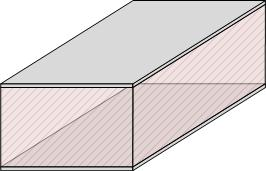
\includegraphics[scale=0.8]{../jpg/ppw.jpg}
\end{center}
\caption{Two infinite planes charged with positive surface charge density $\rho_S$ and $-\rho_S.$}
\label{fig:ParallePlateCapacitorPlain}
\end{figure}

The electric field in an actual parallel-plate capacitor is shown in Figure 

\begin{figure}[htbp]
\begin{center}
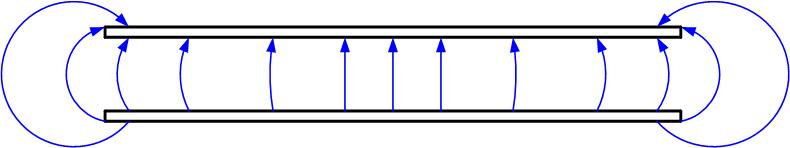
\includegraphics[scale=0.5]{../jpg/Fringing_Fields_For_Finite_Capacitor.jpg}
\end{center}
\caption{Fringing fields in a parallel-plate capacitor. The bottom plate is positively charged, and the top plate is negatively charged.}
\label{fig:FiringinFields}
\end{figure}

The condition that d<<S allows us to ignore fringing fields at the edge of the capacitor, and to assume that the field is equal to the field of two infinite parallel plates of charge. This means that the field is constant in between the plates, oriented from positive to negative plate and zero outside of the plates, as shown in Figure \ref{fig:ParallePlateCapacitorCircuit}.  


\begin{figure}[htbp]
\begin{center}
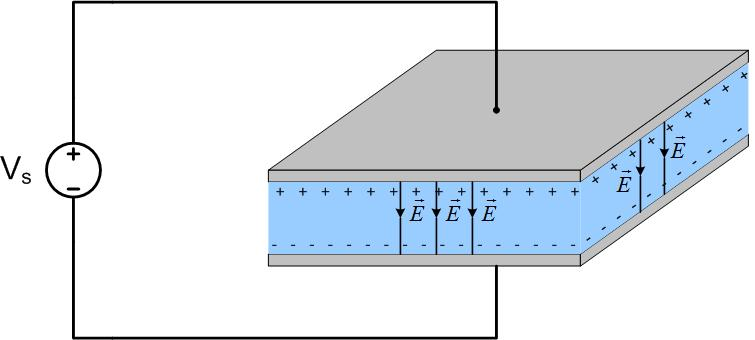
\includegraphics[scale=0.6]{../jpg/Parallel_Plate_Capacitor.jpg}
\end{center}
\caption{Two infinite planes charged with positive surface charge density $\rho_S$ and $-\rho_S.$}
\label{fig:ParallePlateCapacitorCircuit}
\end{figure}


To find the electric field inside the capacitor, we apply Gauss's law to a cylinder whose bottom half is in the dielectric, with the bottom base at the point where we want to find the field, and the top half is in the air above one of the charged plates as shown in Figure \ref{fig:ParallePlateCapacitorGauss}. We see that the flux through the capacitor exists only through the bottom base. The flux through the top base is zero because the field outside the capacitor is zero, and the flux through the side of the cylinder is zero because the electric field does not not go through that surface (in other words the angle between the field and the normal to the surface is $90^o$, and therefore the dot product is zero.) Mathematically, we start from the Gauss's law, assuming that the dielectric permeability is $\epsilon=\epsilon_o \epsilon_r$, where $\epsilon_r$ is the dielectric constant of the material between capacitor's plates.

\begin{equation}
\oint_S \vec{E} \cdot \vec{dS} = \frac{Q_{inS}}{\epsilon}
\end{equation}
 
We split the cylindrical surface S into two base surfaces and a side surface.
 
\begin{equation}
\oint_S \vec{E} \cdot \vec{dS} = \int_{S1}  \vec{E} \cdot \vec{dS} +\int_{S2}  \vec{E} \cdot \vec{dS}+\int_{S3}  \vec{E} \cdot \vec{dS} 
\end{equation}



The dot product between the electric field and the normal to the cylindrical top (S3) surface is zero, because electric field is zero outside of the capacitor. The dot product is zero on the side surface because there is no flux through it, the normal to the surface and the electric field are perpendicular $\vec{E} \cdot \vec{dS}= E \,dS  \cos(\angle(\vec{E},\vec{dS}))= E \,dS  \cos(\angle(90^o)) =0$. The flux through the bottom surface (S1) is just the product of the magnitudes of E and dS $\vec{E} \cdot \vec{dS}= E \,dS  \cos(\angle(\vec{E},\vec{dS}))= E \,dS  \cos(\angle(0^o)) =E dS$, because the normal to the surface and the electric field are in the same direction. We can now take the electric field outside of the integral,   and the integral around the closed surface then becomes
 
 

\begin{equation}
E \int_{S1} dS  = \frac{Q_{inS}}{\epsilon}
\end{equation}

 The integral of surface S1  is just the surface area of the bottom surface.
 
\begin{eqnarray}
E \, S = \frac{Q_{inS}}{\epsilon} \\
 E=\frac{Q_{inS}}{ \epsilon S}
\end{eqnarray}

In the above equation, the ration $\frac{Q_{inS}}{S}$ is just the surface charge density $\sigma$. The final electric field expression for the infinite sheet of charge should include the unit vector of the direction of the field. We will assume that the z-axis is in the up direction from the bottom to the top plate. The field is then

\begin{eqnarray}
 \vec{E}  = \frac{\sigma}{ \epsilon } (-\vec{z})
\end{eqnarray}




\begin{figure}[htbp]
\begin{center}
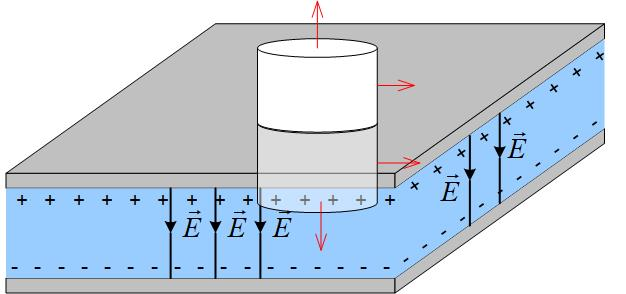
\includegraphics[scale=0.8]{../jpg/Parallel_Plate_Capacitor2.jpg}
\end{center}
\caption{Two infinite planes charged with positive surface charge density $\rho_S$ and $-\rho_S.$}
\label{fig:ParallePlateCapacitorGauss}
\end{figure}


Now that we found the electric field of the paralle plate capacitor, we need to find the potential difference between the two plates, from positive to negative plate. The positive plate in this case is the top plate, so we integrate from d to 0. The potential is defined as 

\begin{equation}
V_{ab}= \int_d^0 \vec{E} \cdot \vec{dl}
\end{equation}


We will find the potential from the bottom plate at z=0 to the top plate at z=d. In the equation above $\vec{dl}$ will always

\begin{eqnarray}
V_{ab}= \int_d^0   \frac{\sigma}{ \epsilon } (\text{-} \vec{z}) \cdot dz \vec{z} \\
V_{ab}= \text{-} \frac{\sigma}{ \epsilon } \int_d^0     \, dz \\
V_{ab}=\frac{\sigma}{ \epsilon } d
\end{eqnarray}

This potential should be positive, because we integrated from the higher to the lower potential. The potential at a lower plate is lower than the potential at the higher plate. If you make a mistake and get a negative potential, it just means you should have started from the positive plate and integrated to the negative plate to get the positive potential difference. However, the $V_{ba}=-V{ab}$, so we can just take the magnitude of the negative potential difference. {\it If the potential difference is a $\log x$ function, make sure that the $x>1$}. The total charge on one plate is $Q=\sigma S$, where S is the area of the plates. The capacitance is then


\begin{eqnarray}
C=\frac{Q}{V} \\
C=\frac{\sigma S}{\frac{\sigma }{ \epsilon } d } \\
C=\epsilon  \frac{S}{d}
\end{eqnarray}


\begin{question}  
The potential difference between the plates of a capacitor is  V. The distance between the plates is d. Ignore fringe effects. The magnitude of the electric field between the plates is:
 
\begin{multipleChoice}  
\choice{not enough information}  
\choice{$V^2/d$}  
\choice{$d/V$}  
\choice[correct]{$V/d$}  
\choice{$d/V^2$}  
\end{multipleChoice}  
\end{question} 



\begin{question}  
The area of the plates of a parallel-plate capacitor is doubled, the capacitance is 

 
\begin{multipleChoice}  
\choice{not enough information}  
\choice{stays the same}  
\choice{quartered}  
\choice{halved}  
\choice[correct]{doubled} 
\end{multipleChoice}  
\end{question} 
If the area of the plates of a parallel-plate capacitor is doubled, the capacitance is 


\section{Coaxial-Cable Capacitance}

Coaxial cable consists of a solid  inner conductor and a conductive outer shell, Figure \ref{fig:coaxialCapacitorGaussInside}.


\begin{figure}[htbp]
\begin{center}
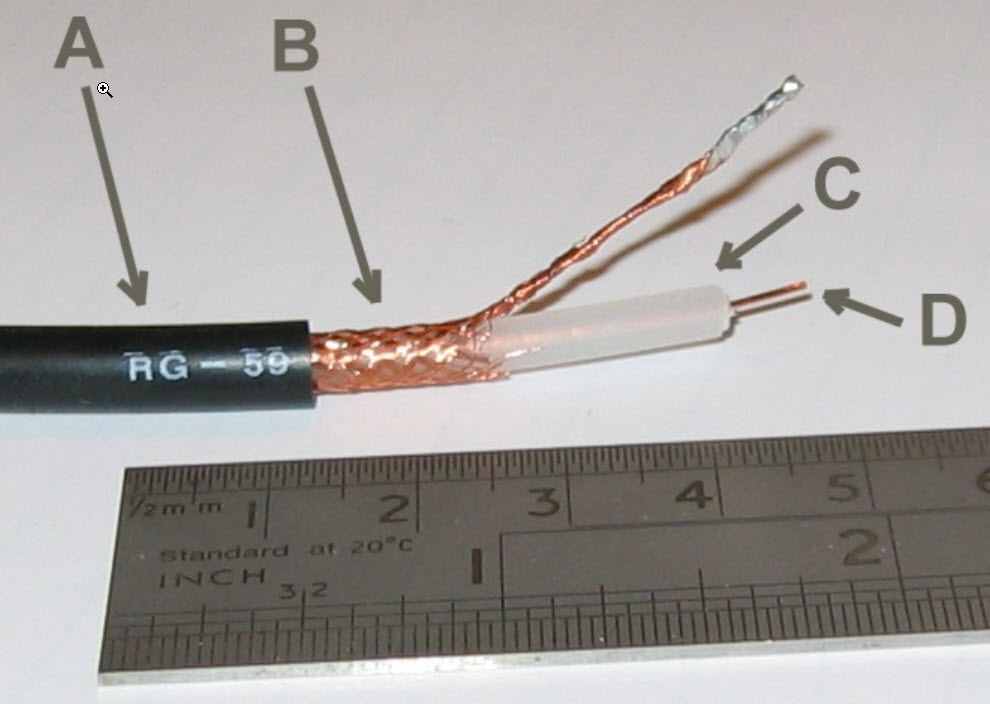
\includegraphics[scale=0.3]{../jpg/coaxialCable.jpg}
\end{center}
\caption{\href{https://en.wikipedia.org/wiki/Coaxial_cable}{A coaxial cable. A - insulator, B - outer conductor, C - dielectric, D - inner conductor. Click to see the Wikipedia page on coaxial cables. } }
\label{fig:coax}
\end{figure}


If we apply Gauss's law to a cylinder outside of the outer conductor, as shown in Figure \ref{fig:coaxialCapacitorGaussOutside}, we see that the field is zero, because the total charge enclosed is zero. 

\begin{figure}[htbp]
\begin{center}
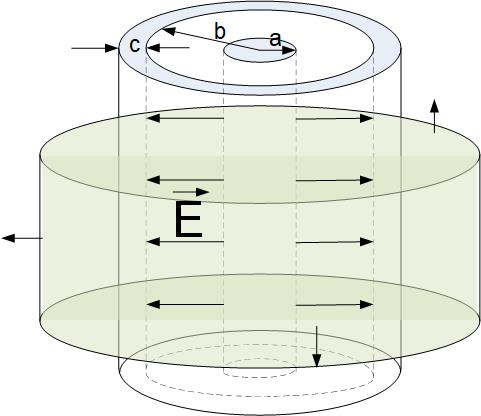
\includegraphics[scale=0.5]{../jpg/coax2.jpg}
\end{center}
\caption{A coaxial cable, with inner conductor charged with positive scharge $Q$ and outer conductor charged with $-Q.$}
\label{fig:coaxialCapacitorGaussOutside}
\end{figure}


 To find the capacitance we need to find the electric field between the inner and outer conductor of a coax. We apply Gauss's law to the green closed cylindrical surface shown in  Figure \ref{fig:coaxialCapacitorGaussInside}. Following the steps in the section on finding the field around the infinite line of charge, we find the field inside the capacitor.
 
 \begin{eqnarray}
 E \, S = \frac{Q_{inS}}{\epsilon} \\
 E=\frac{Q_{inS}}{2 \pi h \epsilon r }
 \end{eqnarray}
 
 To find the potential, we integrate from the inner to the outer conductor.
 
 
 \begin{eqnarray}
 V=\int_a^b \vec{E} \cdot \vec{dr} \\
 V = \int_a^b \frac{Q_{inS}}{2 \pi h \epsilon r } \hat{r} \, \,dr \hat{r} \\
 V=\frac{Q_{inS}}{2 \pi h \epsilon  } \log{\frac{b}{a}}
 \end{eqnarray}
 
 The capacitance is then
 
 \begin{eqnarray}
 C=\frac{Q}{V} \\
 C=\frac{Q}{\frac{Q_{inS} \log{\frac{b}{a}}}{2 \pi h \epsilon  }}\\
 C=\frac{2 \pi h \epsilon} {\log{\frac{b}{a}}} \\
 C'=\frac{C}{h} \\
 C'=\frac{2 \pi  \epsilon} {\log{\frac{b}{a}}}
 \end{eqnarray}

\begin{figure}[htbp]
\begin{center}
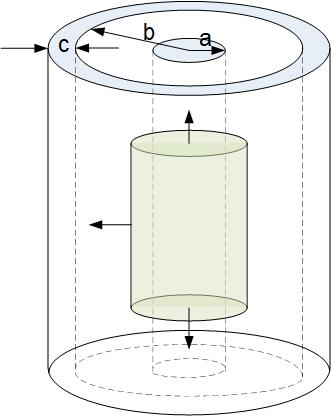
\includegraphics[scale=1]{../jpg/coax1.jpg}
\end{center}
\caption{A coaxial cable, with inner conductor charged with positive scharge $Q$ and outer conductor charged with $-Q.$}
\label{fig:coaxialCapacitorGaussInside}
\end{figure}

Use the calculator below to find the capacitance of RG6 Coaxial Cable, made by Mouser, part number 40001. See \href{https://www.tme.eu/Document/151b7fc68e82e16d70ee1f3bf3c18100/M_004-005-006-007_RG-coaxial_cables.pdf}{data sheet here.} Assume PE dielectric constant is 2.25. Compare with the value in the data sheet.

\geogebra{whkrg2pu}{800}{600}

\section{Spherical Capacitance}

Our earth is a giant spherical capacitor, with ground as one electrode and the ionosphere as another.  Spherical capacitor in Figure \ref{fig:sphericalCapacitor} consists of two concentric shells with radii a and b. The thickness of the outer shell is c-b.  The inner shell is charged with charge Q and outer shell charged with charge -Q. If we apply Gauss's Law to a sphere larger than c, we see that the total charge enclosed is zero, and the field must be zero as well. Between the plates, the field is oriented radially from the positive to the negative charge. Application of Gauss's law to a sphere of a radius r between radii a and b leads to the following equation

\begin{eqnarray}
E\,S = \frac{Q}{\epsilon}
\end{eqnarray}

The surface area of the sphere is $4 \pi r^2$.


\begin{eqnarray}
E 4 \pi r^2 = \frac{Q}{\epsilon} \\
\vec{E}=\frac{Q}{4 \pi \epsilon r^2} \hat{r}
\end{eqnarray}

The potential difference between the inner and outer shell is


\begin{eqnarray}
V=\int_a^b  \vec{E} \cdot  \hat{dr} \\
V=\int_a^b \frac{Q}{4 \pi \epsilon r^2} \hat{r} \,\, dr \hat{r} \\
V=-\frac{Q}{4 \pi \epsilon} \frac{1}{r}|_a^b \\
V=\frac{Q}{4 \pi \epsilon} \frac{b-a}{ab}
\end{eqnarray}

The capacitance is then


\begin{eqnarray}
C=\frac{Q}{V} \\
C=4 \pi \epsilon \frac{ab}{b-a}
\end{eqnarray}

\begin{figure}[htbp]
\begin{center}
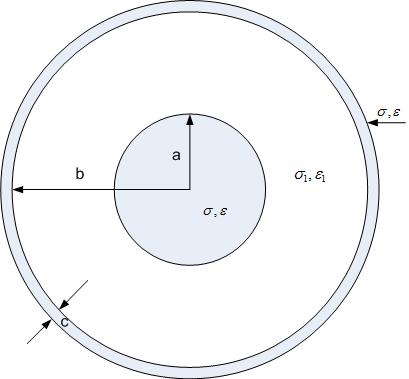
\includegraphics[scale=1]{../jpg/sphereandcylcc.jpg}
\end{center}
\caption{A spherical capacitor, with inner conductor charged with positive scharge $Q$ and outer conductor charged with $-Q.$}
\label{fig:sphericalCapacitor}
\end{figure}


\section{Electrostatic energy of a charged capacitor}

Electrostatic energy is defined as

\begin{equation}
W_e=\frac{1}{2} \int_V \epsilon E^2 dv
\end{equation}

Energy of a charged capacitor can be expressed by any of the following equations

\begin{eqnarray}
W_e=\frac{1}{2} CV^2 \\
W_e=\frac{1}{2} QV \\
W_e=\frac{1}{2} \frac{Q^2}{C} 
\end{eqnarray}

From the definition of electrostatic energy, and the expression for energy of a charged capacitor, we can find the capacitance:

\begin{equation}
C=\frac{Q^2}{\int_V \epsilon E^2 dv} \label{eq:capacitanceEn}
\end{equation}

You can try and solve the capacitance for the above problems again, by using the Equation \ref{eq:capacitanceEn}.

Now, watch the  videos below to experience the energy stored in a charged capacitor, and see  how a fuse and camera flash work by discharging a capacitor.

Do not attempt these demonstrations at home, touching the capacitor's electrodes can be fatal, as humans are good conductors of electricity. Demonstrations were performed at MIT by Prof. Emeritus Walter Lewin.

\begin{center}  
\youtube{ED-Aelxm13A}  
\end{center}


\begin{center}  
\youtube{_cx-PUh2Q7A}  
\end{center} 

\end{document} 
